% !TEX TS-program = pdflatex
% !TEX encoding = UTF-8 Unicode


\documentclass[xcolor=dvipsnames]{beamer}

\usetheme{Boadilla}
%\useoutertheme{miniframes} % Alternatively: miniframes, infolines, split
%\useinnertheme{circles}

\usecolortheme[named=YellowOrange]{structure}
\usepackage{xcolor}
\usepackage{amsmath,amssymb,mathtools}
\usepackage{outlines}
\usepackage{graphicx} % support the \includegraphics command and options
\usepackage{subfigure} %for making subfigures (multiple images in one figure)
\usepackage{pgfplots}
\usepackage[linesnumbered, ruled, vlined, commentsnumbered]{algorithm2e}
\usepackage[center]{caption}
\usepackage{bm}
\usepackage{listings}
\usepackage{minted}
\usepackage{hyperref}
\usepackage{cclicenses} 
\usepackage{comment}

%\beamertemplatenavigationsymbolsempty
%\setbeamertemplate{footline}[frame number]
\usepackage{tikz}
\usetikzlibrary{shapes.misc}
\tikzset{rect/.style={to path={-| (\tikztotarget) -| (\tikztostart) (\tikztotarget)}}}
\usepackage{pgf}
\logo{\pgfputat{\pgfxy(0,7.5)}{\pgfbox[right,base]{
\includegraphics[height=1cm]{NCI_logo.png}}}}
\newcommand{\nologo}{\setbeamertemplate{logo}{}}


\setbeamertemplate{caption}[numbered]

\usepackage[english]{babel}
% or whatever

\usepackage[utf8]{inputenc}
% or whatever

\usepackage{times}
\usepackage[T1]{fontenc}
% Or whatever. Note that the encoding and the font should match. If T1
% does not look nice, try deleting the line with the fontenc.


\title[NCI Training \cc]{Introduction to MPI}% (optional, use only with long paper titles)
%{Resiliency in the Design of Multigrid Method with Adaptively Refined Mesh}


 \author[Fred Fung]{ \\ Frederick Fung}% [Auther, Another] % (optional, use only with lots of authors)


\institute[NCI] % (optional, but mostly needed)
{
  National Computational Infrastructure, Australia
}
% - Use the \inst command only if there are several affiliations.
% - Keep it simple, no one is interested in your street address.

\date[2022] % (optional, should be abbreviation of conference name)
{ \textit{Prepared based on MPI Standard 4.0}}

% - Not really informative to the audience, more for people (including
%   yourself) who are reading the slides online


\lstset{language=C,keywordstyle={\bfseries \color{blue}}}


\begin{document}

\begin{frame}
  \titlepage
\end{frame}

\begin{frame}
$$\textbf{Acknowledgement of Country}$$
The National Computational Infrastructure acknowledges, celebrates and pays our respects to the Ngunnawal and Ngambri people of the Canberra region and to all First Nations Australians on whose traditional lands we meet and work, and whose cultures are among the oldest continuing cultures in human history.
\end{frame}

\begin{frame}
$$\textbf{Disclaimer}$$
This work represents the view of the author delivering this workshop. 
\end{frame}


\begin{frame}{Outline}
\begin{block}{Goal}
This two half-day workshop consists of lectures and coding exercises. The goal of this session is to get users familiar with a broad range of common communication mechanisms offered by the MPI library.
\end{block}

\pause
\begin{block}{Caveat}
Lower your expectations. You are unlikely becoming an MPI expert after studying one code example. 

(Use LLM of your choice to help write an expert MPI code)
\end{block}
\end{frame}

\begin{frame}{Agenda and Topics Covered}
\begin{outline}
    \1 Day 1
     \2 Syntax and semantics
    \2 Point-to-point communication
    \3 Blocking communication
    \3 Non-blocking communication
    \3 Overlapping communication with computation
    \3 Persistent communication 
    \1 Day 2
     \2Collective communication
    \2 One-sided communication
    \2 MPI Profiling
    \2 MPI-IO (optional)
\end{outline}
\pause
\begin{block}{}
In this workshop, we will demonstrate each of the communication patterns in a two-dimensional finite difference method example.    
\end{block}
\end{frame}

\begin{frame}{What is MPI}
\begin{outline}
    \1 MPI stands for Message Passing Interface.
    \2 The development of the standardisation is community driven and is derived from state-of-art research by university researchers, vendors of hardware, government laboratories and industry.
    \pause
    \2 There are many implementations of the standard: MPICH, OpenMPI, Intel MPI, Cray MPI, IBM MPI etc.
    \1 MPI is suitable for use by MIMD (multiple instruction multiple data)  or SPMD (single prgroam multiple data) programs.
    \2 Such program usually runs on distributed-memory multiprocessors.
    \pause
    \1 MPI dominates HPC programs \cite{evans2022survey}.
    \2 All responded projects in Exascale Computing Projects\footnote{The US Department of Energy Office of Science and the National Nuclear Security Administration initiated the Exascale
Computing Project (ECP) in 2016 to prepare mission-relevant applications and scientific software for the delivery of the
exascale computers starting in 2023.} use MPI.
\end{outline}
\end{frame}

\begin{frame}{A brief history of the MPI standard}
\small
\begin{outline}
\1 More than 30 years of MPI: the first standard appeared in 1994.
\2 1992: Standardisation work began.
\2 1994: MPI 1.0 --- point-to-point, datatypes and collectives.
\2 1995: MPI 1.1 --- corrections and clarifications.
\2 1997: MPI 1.2 --- clarifications, published with MPI 2.0.
\2 1997: MPI 2.0 --- parallel I/O, RMA and dynamic processes.
\2 2008: MPI 1.3 consolidated MPI-1; MPI 2.1 unified MPI-1 and MPI-2.
\2 2009: MPI 2.2 --- corrections and small additions.
\2 2012: MPI 3.0 --- nonblocking collectives and extended RMA.
\2 2015: MPI 3.1 --- clarifications and nonblocking collective I/O.
\2 2021: MPI 4.0 --- large counts, persistent collectives,\newline
    partitioned communication and Sessions.
\2 2023: MPI 4.1 --- clarifications and minor extensions.
\2 2025: MPI 5.0 --- standard Application Binary Interface (ABI).
\end{outline}
\footnotesize\textit{Adapted from George Bosilca; updated for 2026.}\par
\footnotesize Source: \href{https://www.mpi-forum.org/docs/}{MPI Forum standards and release history}.
\end{frame}

\begin{frame}{Why MPI?}
\begin{outline}
\1 Scalability in parallel computing
\2 Solving $kN$ scale problem with $kN$ computational resources during the same computation time - \textbf{weak scaling}.
\pause
\2 Solving a problem with $kN$ computational resources during $1/k$ computation time - \textbf{strong scaling}.
\end{outline}
\pause
\begin{block}{}
MPI utilises a large number amount of computational resources available to users i.e. making the $kN$ term.
\end{block}
\end{frame}

\begin{frame}{MPI Implementations on Gadi}
On Gadi, two MPI implementations are available by Environment module.
\begin{outline}
\1 Intel MPI e.g. \$module load intel-compiler/[version], \$module load intel-mpi/[version]
\1 OpenMPI e.g. \$module load openmpi/[version]
\end{outline}

Compilation:
\begin{outline}
    \1 Fortran: \$mpi77, mpif90 
    \2 \$ mpif77\\
    \2 \$ mpif90
    \2 \$ mpiifort
    \1 C/C+: 
    \2 \$ mpicc
    \2 \$ mpiicc
\end{outline}
\end{frame}

\begin{frame}{What MPI ISN'T}
\begin{outline}
\1 MPI does
\2 provide you a communication library;
\2 provide you datatypes;
\2 have language bindings with C and Fortran;
\2 provide parallel I/O;
\2 provide interface for tool support;
\2 and many more.
\1 MPI does NOT 
\2 design parallelism for your serial code.
\end{outline}
\pause
\begin{block}{}
Users are responsible for the correctness of the implementation of their parallel algorithms. We use the next example to elaborate.
\end{block}
\end{frame}

\begin{frame}{Example: Monte-carlo Approximation of $\pi$}
\begin{figure}
    \centering
    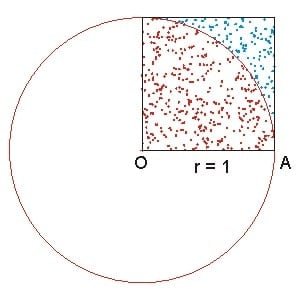
\includegraphics[height=0.6\textheight]{Monte-Carlo01.jpg}
    \caption{Generate $N$ random sampling points within a square, and count the number $h$ of samples that fall in the circle. Then the approximation $\pi \approx 4h/N$  }
    \label{pi}
\end{figure}
\end{frame}

\begin{frame}[fragile]
\frametitle{Example: Monte-Carlo Approximation of $\pi$}
$$\textbf{A serial code}$$
\rule{\textwidth}{1pt}
\scriptsize
\begin{minted}{C}
    seed  = 1; /* seed to generate random numbers */
    for (i=0; i<N; i++){
      x = rand_r(&seed)/ (double) RAND_MAX; /* RAND_MAX to normalise */ 
      y = rand_r(&seed)/ (double) RAND_MAX;

    if (x*x + y*y <= 1.0f) count+=1;
    } 
\end{minted}
\rule{\textwidth}{1pt}
$x,y$ are normalised random numbers. Variable declarations are not shown.
\end{frame}

\begin{frame}[fragile]{Example: Monte-Carlo Approximation of $\pi$}
$$\textbf{Parallel MPI code}$$
\rule{\textwidth}{1pt}
\scriptsize
\begin{minted}{C}
      int rank, size;
      int count=0, count_tot=0
      MPI_Comm_rank(MPI_COMM_WORLD, &rank);
      MPI_Comm_size(MPI_COMM_WORLD, &size);
      int start = rank * N / size;
      int end = (rank+1) * N /size;
      for (i=start; i<end; i++){
        seed = rank;
        x = rand_r(&seed)/ (double) RAND_MAX;
        y = rand_r(&seed)/ (double) RAND_MAX;
        if (x*x + y*y <= 1.0f) count+=1; }
      MPI_Reduce(&count, &count_tot, 1, MPI_INT,
      MPI_SUM, 0, MPI_COMM_WORLD)
\end{minted}
\rule{\textwidth}{1pt}
Users organise the copies of data for each parallel processes.
\end{frame}

 \begin{frame}{Six Mostly Used MPI Calls}
 \begin{outline}
     \1 MPI$\_$INIT\\
     \1 MPI$\_$COMM$\_$RANK\\
     \1 MPI$\_$COMM$\_$SIZE\\
     \1 MPI$\_$SEND\\
     \1 MPI$\_$RECV\\
     \1 MPI$\_$FINALIZE
 \end{outline}
 \end{frame}

\begin{frame}[fragile]{"Start" MPI Process}
\begin{block}{MPI$\_$INIT}
MPI$\_$INIT()
\end{block}

C Binding
\rule{\textwidth}{1pt}
\scriptsize
\begin{minted}{C}
/* initialise MPI */
int MPI_Init(int &argc, char &argv)
\end{minted}
\rule{\textwidth}{1pt}
\end{frame}

\begin{frame}{MPI$\_$INIT}
\begin{outline}
\1 The call does not create a process; rather, it initialises the MPI environment.
\2 e.g defines the initial communicator MPI$\_$WORLD$\_$COMM.
\1 MPI functions must only be called after this call.
\end{outline}
\end{frame}

\begin{frame}{Communicator}
\begin{outline}
\1 Group of processes for communication.
\1 Communicator must be specified in MPI program as a unit
of communication. 
\2 Default is MPI$\_$WORLD$\_$COMM.
\1 Multiple communicators can be defined, either overlapping or non-overlapping.
\end{outline}
\end{frame}

\begin{frame}{Communicator}
\begin{figure}
    \centering
    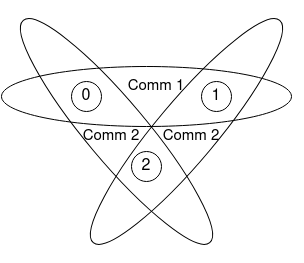
\includegraphics[width=0.6\textwidth]{communicator.png}
    \caption{Overlapping communicators \cite{mpi40}}
\end{figure}
\end{frame}


\begin{frame}[fragile]{Communicator Management}
\begin{block}{MPI$\_$COMM$\_$SIZE}
MPI$\_$COMM$\_$SIZE(\textbf{comm, size})
\\
\begin{itemize}
\item[] IN \textbf{comm} \: \textit{communicator (handle)}\\
\item[] OUT \textbf{size} \: \textit{number of processes in the group of comm (integer)}\\
\end{itemize}
\end{block}

C Binding
\rule{\textwidth}{1pt}
\scriptsize
\begin{minted}{C}
/* determine the number of processes in the group of comm */
int MPI_Comm_size(MPI_Comm comm, int *size)
\end{minted}
\rule{\textwidth}{1pt}
\end{frame}


\begin{frame}[fragile]{Communicator Management}
\begin{block}{MPI$\_$COMM$\_$RANK}
MPI$\_$COMM$\_$RANK(\textbf{comm, rank})
\\
\begin{itemize}
\item[] IN \textbf{comm} \: \textit{communicator (handle)}\\
\item[] OUT \textbf{rank} \: \textit{rank of the calling process in group of comm (integer)}\\
\end{itemize}
\end{block}

C Binding
\rule{\textwidth}{1pt}
\scriptsize
\begin{minted}{C}
/* determine the rank of the calling process in group of comm */
int MPI_Comm_rank(MPI_Comm comm, int *rank)
\end{minted}
\rule{\textwidth}{1pt}
\end{frame}





\begin{frame}[fragile]{"Close" MPI Process}
\begin{block}{MPI$\_$FINALIZE}
MPI$\_$FINALIZE()
\end{block}

C Binding
\rule{\textwidth}{1pt}
\scriptsize
\begin{minted}{C}
/* clean up MPI */
int MPI_Finalize()
\end{minted}
\rule{\textwidth}{1pt}
\end{frame}

\begin{frame}{MPI$\_$FINALIZE}
\begin{outline}
\1 This call does not shut down the processes.
\2 Behaviour could be undefined if called on a process that still participates in communication.
\2 Consider MPI$\_$Abort to capture catastrophic errors.
\end{outline}
\end{frame}


\begin{frame}[fragile]{The structure of a basic MPI program in C}
\rule{\textwidth}{1pt}
\scriptsize
\begin{minted}{C}
#include<stdio.h>
#include<mpi.h>

int main(int argc, char *argv[]){
int rank, size;
MPI_Init(&argc, &argv);
double start_t, end_t;
start_t = MPI_Wtime();
MPI_Comm world = MPI_COMM_WORLD;
MPI_Comm_rank(world, &rank);
MPI_Comm_size(world, &size);

/* codes using the MPI library */

end_t = MPI_Wtime();
 /* optional,for ordered prints only */ 
printf("MPI program runtime = %f on rank %d\n", end_t-start_t, rank);
MPI_Finalize();
\end{minted}
\rule{\textwidth}{1pt}
\end{frame}

\begin{frame}{Exercise}
Review the program MC$\_$pi.c to understand the structure of a basic MPI program.
\end{frame}

\begin{frame}{Model Problem: 2D Poisson Equation}
\begin{block}{}
Consider a two-dimensional Poisson equation with Dirichlet boundary condition over a unit square domain $\Omega = [0,1] \times [0,1]$
\begin{align*}
-\Delta u &= f \; \text{in} \; \Omega \\
 u &= g \; \text{on} \; \partial \Omega
\end{align*}
\end{block}
\end{frame}

\begin{frame}{Model Problem: Discretisation}
\begin{block}{Finite difference}
We use the second-order central finite difference method to discretise the Laplace operator
 \begin{align*}
     \big(\Delta u\big)_{i,j} & = \big(D_{xx}^2u\big)_{i,j}+ \big(D_{yy}^2 u\big)_{i,j}\\[2ex]
     & \approx \frac{u_{i+1,j}-2u_{i,j}+u_{i-1,j}}{h^2} + \frac{u_{i,j+1}-2u_{i,j}+u_{i,j-1}}{h^2} 
 \end{align*}
leading to
\begin{align*}
    -\big(\Delta u)\big)_{i,j} = \frac{4u_{i,j}-u_{i+1,j}-u_{i-1,j}-u_{i,j+1}-u_{i,j-1}}{h^2}=f(u_{i,j}).
\end{align*}
\end{block}
\end{frame}


\begin{frame}{Model Problem: the mesh and the stencil}

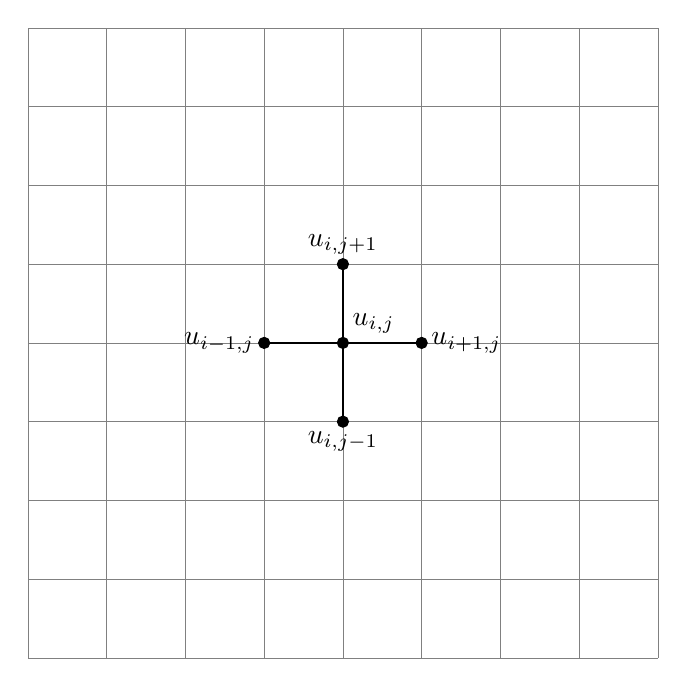
\begin{tikzpicture}
\draw[step=1cm,gray,very thin] (-2,-2) grid (6,6);
\draw[thick,- ] (1,2) -- (3,2);
\draw[thick,- ] (2,1) -- (2,3);
\filldraw (3,2) circle (2pt) node [right] {$u_{i+1, j}$};
\filldraw (2,3) circle (2pt) node [above] {$u_{i, j+1}$};
\filldraw (1,2) circle (2pt) node [left] {$u_{i-1, j}$}; 
\filldraw (2,1) circle (2pt) node [below] {$u_{i, j-1}$};
\filldraw (2,2) circle (2pt) node [above right ] {$u_{i,j}$};
\end{tikzpicture}
\end{frame}

\begin{frame}{Model Problem: Parallelisation}
\begin{block}{Domain decomposition}
Users are responsible to decompose the mesh for parallelsiation. For simplicity, the mesh is decomposed vertically in our practice code. Further,  unless otherwise stated,  we assume the mesh is split into upper submesh and the lower submesh and are distributed to two processes respectively.
\end{block}
\end{frame}

\begin{frame}{Model Problem: Parallelisation}
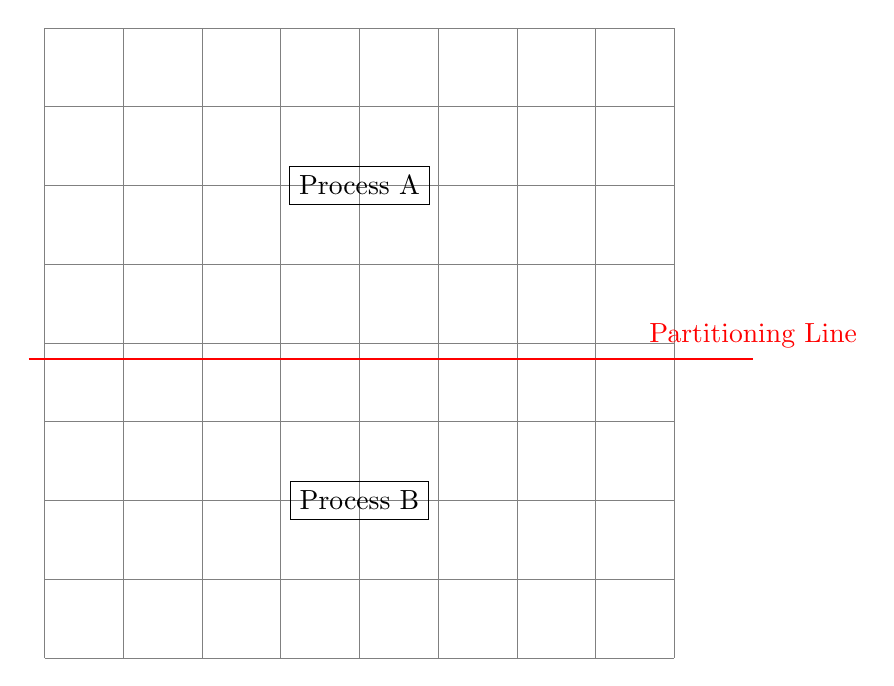
\begin{tikzpicture}
\draw[step=1cm,gray,very thin] (-2,-2) grid (6,6);
\draw[thick,-, color=red] (-2.2,1.8) -- (6.2,1.8);
\node[draw] at (2,4) {Process A};
\node[draw] at (2,0) {Process B};
\draw[thick,-, color=red] (-2.2,1.8) -- (7,1.8) node [above] {Partitioning Line};
\end{tikzpicture}
\end{frame}

\begin{frame}{Model Problem: Ghost nodes vs Full nodes }

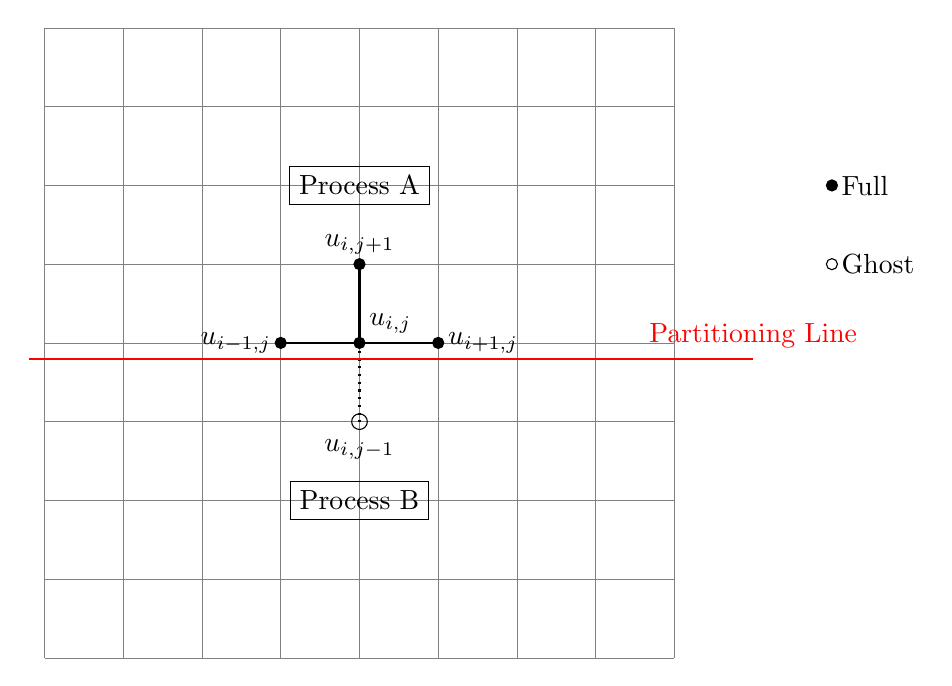
\begin{tikzpicture}[
  circ/.style={shape=circle, inner sep=2pt, draw, node contents=}]
\draw[step=1cm,gray,very thin] (-2,-2) grid (6,6);
\draw[thick,- ] (1,2) -- (3,2);
\draw[thick,-, dotted ] (2,2) -- (2,1);
\draw[thick,-] (2,2) -- (2,3);
\draw[thick,-, color=red] (-2.2,1.8) -- (7,1.8) node [above] {Partitioning Line};
\node[draw] at (2,4) {Process A};
\node[draw] at (2,0) {Process B};
%\draw at (8,4) (1pt)  circle node {Full};
\filldraw (8,4) circle (2pt) node [right] {Full};
\draw (8,3) circle (2pt) node [right] {Ghost};
\filldraw (3,2) circle (2pt) node [right] {$u_{i+1, j}$};
\filldraw (2,3) circle (2pt) node [above] {$u_{i, j+1}$};
\filldraw (1,2) circle (2pt) node [left] {$u_{i-1, j}$}; 
%\filldraw (2,1) circle (2pt) node [below] {$u_{i, j-1}$};
\filldraw (2,2) circle (2pt) node [above right ] {$u_{i,j}$};
\node[draw] at (2, 1) (2pt) [circ, label=below:{$u_{i, j-1}$}];
%\draw (2,1) node[cross=5pt,rotate=10, red] {};
\end{tikzpicture}
\end{frame}

\begin{frame}{}
    \textbf{Problem: How to exchange the ghost node information between Process A and B?}
\end{frame}



\begin{frame}
    $$\textbf{Topic 1: Syntax and Semantics}$$
\pause
$$\textcolor{red}{\textbf{Warning: It does get tedious}}$$
\end{frame}


\begin{frame}{Semantics}
\begin{outline}
\1 MPI Operations
\1 MPI Procedures
\1 MPI Functions
\end{outline}
\end{frame}

\begin{frame}
\begin{columns}[T] % align columns
\begin{column}{.48\textwidth}
\begin{outline}
\1 MPI Operations
\1 MPI Procedures
\1 MPI Functions
\end{outline}
\end{column}%
\hfill%
\begin{column}{.48\textwidth}
\begin{figure}
    \centering
    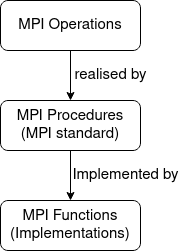
\includegraphics[width=0.8\textwidth]{MPI_operation.png}
    \label{standard_send}
\end{figure}
\end{column}% 
\end{columns}
\end{frame}

\begin{frame}{MPI Operations }
\begin{block}{Definition \cite{mpi40}}
An MPI operation is a sequence of steps performed by the MPI library to
establish and enable data transfer and/or synchronisation. It consists of four stages:
\textbf{initialisation}, \textbf{starting}, \textbf{completion}, and \textbf{freeing}, and it is implemented as a set of one or more MPI procedures.
\end{block}

\begin{outline}
\1 Blocking operations 
\1 Nonblocking operations
\1 Persistent operations
\1 Collective operations
\end{outline}

\begin{block}{Remark}
An MPI operation describes the property of a class of data transfer mechanism but does not define a unique MPI procedure.
\end{block}
\end{frame}

\begin{comment}
\begin{frame}
\begin{block}{Initialisation}
     Hands over the argument list to the operation but not the content of the data buffers.
\end{block}
\begin{block}{Starting}
Hands over the control of the data buffers, if any, to the associated operation.
\end{block}
\begin{block}{Completion}
Returns control of the content of the data buffers and indicates that
output buffers and arguments, if any, have been updated.
\end{block}
\begin{block}{Freeing}
Returns control of the rest of the argument list.
\end{block}
\end{frame}
\end{comment}

\begin{frame}
\begin{block}{Definition Blocking operation}
All four stages are combined in a single procedure call.
\end{block}
\begin{figure}
    \centering
    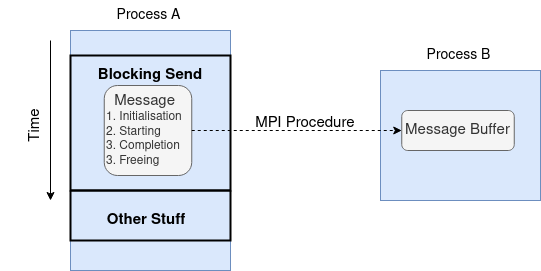
\includegraphics[width=\textwidth]{Blocking_Send.png}
    \caption{The send operation is blocking at process A }
\end{figure}
\end{frame}

\begin{frame}
\begin{block}{Definition Nonblocking operation}
The initialization and starting stages are combined into a single nonblocking procedure call and the completion and
freeing stages are combined into a separate, single procedure call.
\end{block}
\begin{figure}
    \centering
    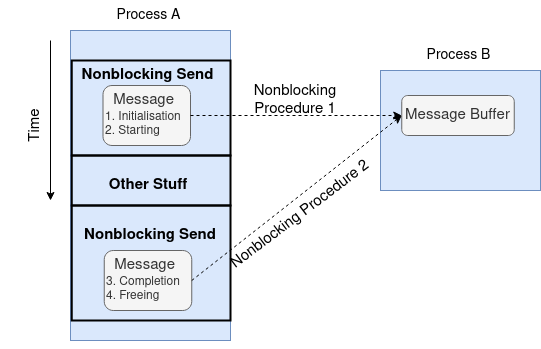
\includegraphics[width=0.8\textwidth]{NonBlocking_Send.png}
    \label{standard_send}
\end{figure}
\end{frame}

\begin{frame}
\begin{block}{Definition Persistent operation}
There is a separate procedure for each of the four stages. 
\end{block}
\begin{figure}
    \centering
    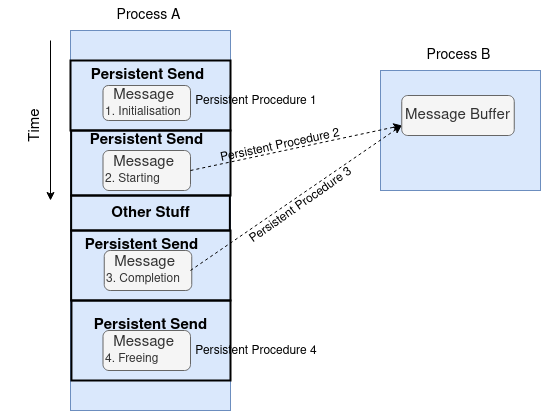
\includegraphics[width=0.8\textwidth]{Persistent_Send.png}
    \label{standard_send}
\end{figure}
\end{frame}


\begin{frame}{MPI Procedures}
\begin{block}{Definition}
MPI procedures describe functionalities and are specified using a language-independent notation. An MPI
operation-related procedure implements at least a part of a stage of an MPI operation.
\end{block}
\begin{outline}
\1 Examples
\2 MPI$\_$SEND, MPI$\_$PROBE (>400) (Note all letters are capitalised)
\end{outline}
\begin{block}{}
All MPI procedures can either be local or non-local: Whether its returning requires it to be called on another MPI Process.
\end{block}
\end{frame}

\begin{frame}{MPI Functions}
\begin{block}{Definition}
In this workshop, MPI functions are MPI procedures implemented by MPI implementations with language bindings.
\end{block}
\begin{outline}
\1 Example
\2 MPI$\_$Send, MPI$\_$Probe etc
\end{outline}
\end{frame}

\begin{frame}
We summarise the semantics with the send operation example.
\begin{figure}
    \centering
    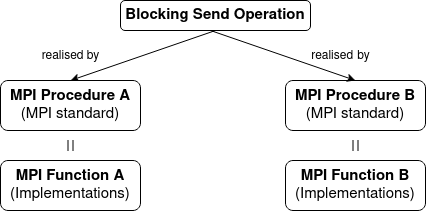
\includegraphics[width=0.8\textwidth]{Blocking_operation.png}
    \label{standard_send}
\end{figure}
\end{frame}

\begin{frame}
With the nonblocking send example.
\begin{figure}
    \centering
    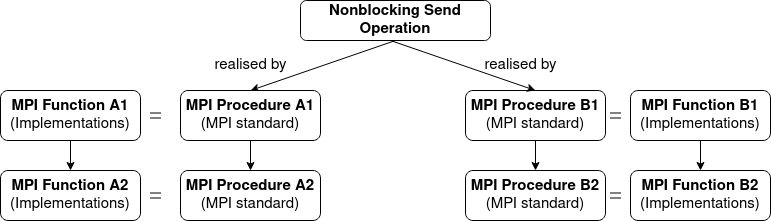
\includegraphics[width=0.8\textwidth]{Nonblocking_operation.png}
    \label{standard_send}
\end{figure}
\end{frame}

\begin{frame}{}
$$\textbf{Topic 2: Point-to-point Communication}$$
\end{frame}

\begin{frame}{What is a message?}
$$\textbf{Message = Message data + Message envelope}$$
\begin{block}{Message date}
$$\textit{ (address, count, datatype)}$$
Information consists of count successive entries of the type indicated by datatype, starting with the entry at address buffer.
\end{block}

\begin{block}{Message envelope}
$$\textit(source, destination, tag, communicator)$$
Information that can be used to distinguish
messages and selectively receive them.
\end{block}
\end{frame}

\begin{frame}[fragile]{What is a message?}
\begin{outline}
    \1 \textit{datatype}: A predefined name to specify machine-independent data elements.
    \2 Basic datatypes: MPI$\_$INT, MPI$\_$DOUBLE (in C); MPI$\_$INTEGER, MPI$\_$REAL (in Fortran).
    \2 Derived datatypes: mix of basic datatypes.
    \2 MPI datatype is not an actual datatype in the host language.
    \2 Data can be communicated between machines with different memory representations.
    \1 \textit{tag}: distinguishes different types of messages.
    \1\textit{communicator}: specifies a "communication universe". Messages are always received within the "communication universe" they were sent, and messages sent in different "communication universe" do not interfere.
    \2 MPI$\_$COMM$\_$WORLD: communication within all processes available at initialisation time.
\end{outline}
\end{frame}

\begin{frame}[fragile]{}
\begin{figure}
    \centering
    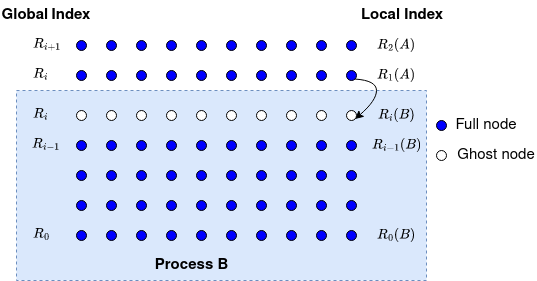
\includegraphics[width=0.7\textwidth]{Submesh.png}
    \caption{The message of row $i$ is sent from Process A and received by Process B}
    \label{send-recv}
\end{figure}
\rule{\textwidth}{1pt}
\scriptsize
\begin{minted}{C}
MPI_Send(submesh[1], mesh_size, MPI_DOUBLE, lower, lowertag,\
MPI_COMM_WORLD);
\end{minted}
\rule{\textwidth}{1pt}
\end{frame}





% \begin{frame}{Six Mostly Used MPI Calls (i.e. most users only use those six calls)}
% \begin{enumerate}
%     \item MPI\_INIT\\
%     \item MPI\_COMM\_RANK\\
%     \item MPI\_Comm\_Size\\
%     \item MPI\_Send\\
%     \item MPI\_Recv\\
%     \item MPI\_Finalize
% \end{enumerate}
% \end{frame}

\section{Point-to-point communication}

\begin{frame}{Topic 1A: Blocking Communication}
\begin{outline}
    \1 Blocking SEND-RECV is the basic MPI communication mechanism.
\end{outline}
\end{frame}


\begin{frame}{Topic 1A: Blocking Send Communication}
\begin{figure}
    \centering
    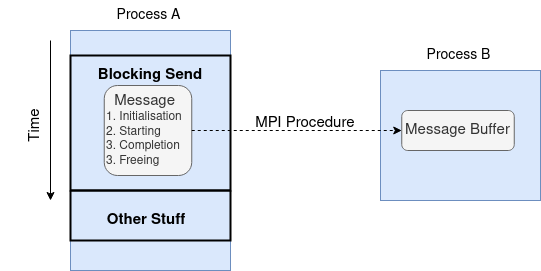
\includegraphics[width=\textwidth]{Blocking_Send.png}
    \caption{A simplified schematic diagram: the data message is sent from process A and received by process B through a communication network.}
    \label{send-recv}
\end{figure}
\end{frame}

\begin{frame}
\begin{block}{Definition 1. Blocking Operation}
All four stages are combined in a single
procedure call.
\end{block}

\begin{block}{Definition 2. Blocking Send}
The corresponding MPI procedure does not return until the message
data and envelope have been safely stored away so that the sender is free to modify the
send buffer.
\end{block}

$$\textit{Definition 1} \implies \textit{Definition 2}$$
\end{frame}

\begin{frame}{Communication modes}
\begin{block}{Remark}
For the blocking send, the message might be sent directly into the matching receiver's buffer or it might be copied into a temporary system buffer. MPI offers the following \textbf{communication modes} for users to choice how they want to complete the blocking. 
\end{block}
\begin{outline}
    \1 Standard Send
    \1 Buffered Send
    \1 Synchronous Send
    \1 Ready Send 
\end{outline}
\end{frame}

\begin{frame}{Communication delayed}
\begin{figure}
    \centering
    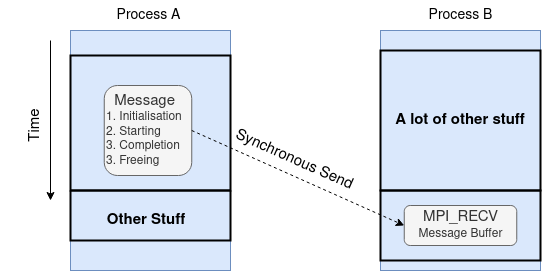
\includegraphics[width=0.8\textwidth]{MPI_Send_delay.png}
    \caption{The SEND from processor A is held until the matching RECV is posted in processor B.}
    \label{send-recv}
\end{figure}
\end{frame}


\begin{frame}{MPI$\_$SEND (Standard mode)}
\begin{figure}
    \centering
    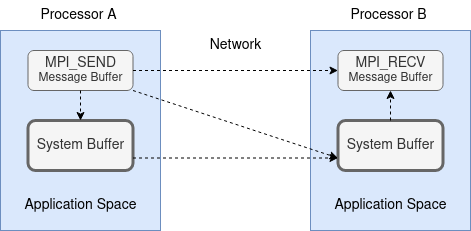
\includegraphics[width=0.6\textwidth]{Standard_send.png}
    \caption{The standard mode either buffers the outgoing data or sends to the matching receiver - up to the MPI implementation to decide.}
    \label{standard_send}
\end{figure}
\end{frame}

\begin{frame}[fragile]{MPI$\_$SEND (Standard mode)}
\begin{block}{MPI$\_$SEND}
MPI$\_$SEND(\textbf{buf, count, datatype, dest, tag, comm})
\\
\begin{itemize}
\item[] IN \textbf{buf} \: \textit{starting address of buffer (choice)}\\
\item[] IN \textbf{count} \: \textit{number of entries in buffer (non-negative integer)}\\
\item[] IN \textbf{datatype} \: \textit{datatype of elements in send buffer (handle)}\\
\item[] IN \textbf{dest} \: \textit{rank of destination(integer)}\\
\item[] IN \textbf{tag} \: \textit{message tag (integer)}\\
\item[] IN \textbf{comm} \: \textit{communicator (handle)}\\
\end{itemize}
\end{block}

C Binding
\rule{\textwidth}{1pt}
\scriptsize
\begin{minted}{C}
/* A buf message is sent from the calling rank to destination rank */
int MPI_Send(const void *buf, int count, MPI_Datatype datatype, int dest,
int tag, MPI_Comm comm)
\end{minted}
\rule{\textwidth}{1pt}
\end{frame}

\begin{frame}{MPI$\_$SEND (Standard mode)}
\begin{outline}
    \1 Blocking operations implies that neither the send buffer nor the argument list can be modified until the buffer is safely stored somewhere.
    \1 System buffer may be outside the application space.
    \1 How system buffer would be chosen is up to particular MPI implementations.
    \1 Eager protocol - small messages.
    \1 Rendezvous protocol - large messages.
    \1 It may complete before the matching RECV is posted.
\end{outline}
\end{frame}


\begin{frame}{MPI$\_$BSEND (Buffer mode)}
\begin{figure}
    \centering
    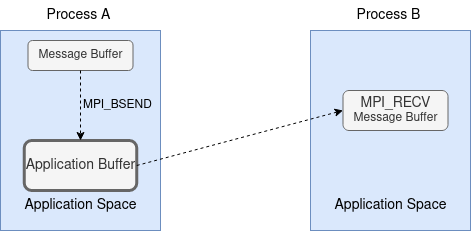
\includegraphics[width=0.6\textwidth]{Buffer_send.png}
    \caption{The buffer mode buffers the message to the application buffer provided by the user.}
    \label{buffer_send}
\end{figure}
\end{frame}

\begin{frame}{MPI$\_$BSEND (Buffer mode)}
\begin{outline}
\1 Users are responsible to provide enough space for buffer.
\1 Only one buffer is allowed in a process at a time.
\1 The implementation varies.
\1 Be cautious to use this call.
\end{outline}
\end{frame}

\begin{frame}{MPI$\_$SSEND (Synchronous mode)}
\begin{figure}
    \centering
    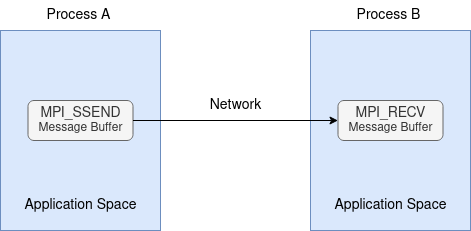
\includegraphics[width=0.6\textwidth]{Sync_send.png}
    \caption{The communication does not complete at either end before both
processes rendezvous at the communication.}
\end{figure}
\end{frame}

\begin{frame}{MPI$\_$SSEND (Synchronous mode)}
\begin{outline}
\1 MPI$\_$SSEND 
\2 Completes only if a matching receive is posted, and the receiver has started to receive the message.
\2 Implies the sender has to hold until a matching receive is posted, and the receiver has started to receive the message before continuing. 
\2 Ensures synchronisaton:  both processes have reached a certain point.
\2 Counter-intuitively, this call has no implication for buffering.
\1 Programmers should treat all sends synchronous, i.e. not rely on buffering to complete.
\end{outline}
\end{frame}



\begin{frame}{An erroneous example: Deadlock}
\begin{figure}
    \centering
    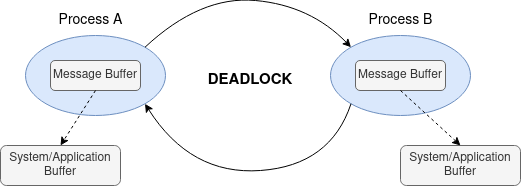
\includegraphics[width=0.8\textwidth]{MPI_deadlock.png}
    \caption{The message sent by each process has to be copied out before the send operation returns and the receive operation starts. For the program to complete, it is necessary that at least one of the two messages sent be buffered. Thus, this program can succeed only if the communication system can buffer at least \textit{count} words of data. \cite{mpi40}}
\end{figure}
\end{frame}



\begin{frame}{MPI$\_$RECV}
\begin{outline}
\1 RECV is asymmetric to SEND in MPI.
\2 A receiver may accept messages from an arbitrary sender.
\2 The length of the RECV buffer can be equal to or greater than the length of the RECV message.
\2 MPI send and receive is a "push" mechanism.
\1 There is only one blocking RECV procedure but matches any of the send modes.
\end{outline}
\end{frame}

\begin{frame}[fragile]{MPI$\_$RECV}
\begin{block}{MPI$\_$RECV}
MPI$\_$RECV(\textbf{buf, count, datatype, source, tag, comm, status})
\\
\begin{itemize}
\item[] IN \textbf{buf} \: \textit{starting address of buffer (choice)}\\
\item[] IN \textbf{count} \: \textit{number of entries in buffer (non-negative integer)}\\
\item[] IN \textbf{datatype} \: \textit{datatype of elements in send buffer (handle)}\\
\item[] IN \textbf{cource} \: \textit{rank of source or MPI$\_$ANY$\_$SOURCE (integer)}\\
\item[] IN \textbf{tag} \: \textit{message tag or MPI$\_$ANY$\_$TAG (integer)}\\
\item[] IN \textbf{comm} \: \textit{communicator (handle)}\\
\item[] OUT \textbf{status} \: \textit{status object (status)}
\end{itemize}
\end{block}

C Binding
\rule{\textwidth}{1pt}
\scriptsize
\begin{minted}{C}
/* A buf message is received at the calling rank */
int MPI_Recv(void *buf, int count, MPI_Datatype datatype, int source, 
int tag, MPI_Comm comm, MPI_Status *status)
\end{minted}
\rule{\textwidth}{1pt}
\end{frame}


\begin{frame}{MPI$\_$RECV}
\begin{outline}
\1 Status in C: is a structure that contains three field named MPI$\_$Source, MPI$\_$TAG, MPI$\_$ERROR\\
\1 Status in Fortran: is an array of integers.
\end{outline}
\end{frame}


\begin{frame}[fragile]{Blocking Send and RECV}
\rule{\textwidth}{1pt}
\scriptsize
\begin{minted}{C}
/* Send the bottom row of full nodes and receive update 
on the top row of ghost nodes */
MPI_Send(submesh[*ptr_rows-2], mesh_size, MPI_DOUBLE, upper, uppertag, 
MPI_COMM_WORLD);
MPI_Recv(submesh[0], mesh_size, MPI_DOUBLE, lower, uppertag,
MPI_COMM_WORLD, &status);

/* Jacobi method iterates on the interior full nodes */
Jacobi(ptr_rows, mesh_size, &submesh[0][0], &submesh_new[0][0],
&subrhs[0][0], space);

\end{minted}
\rule{\textwidth}{1pt}
See the complementary code for details.
\end{frame}

\begin{frame}{}
\begin{figure}
    \centering
    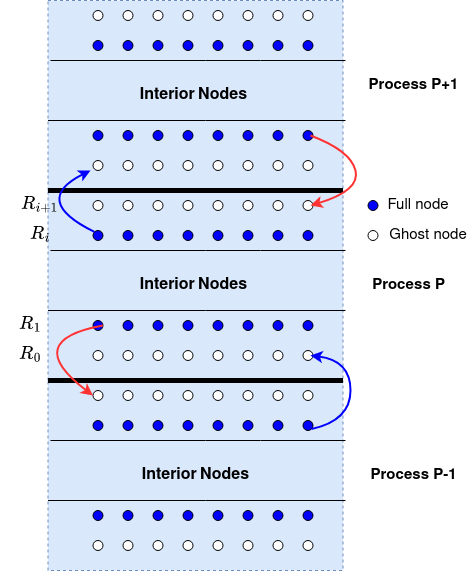
\includegraphics[width=0.5\textwidth]{MPI_Communicate.png}
    \caption{The communication of ghost nodes between processes.}
\end{figure}
\end{frame}


\begin{frame}{Exercise}
In laplace$\_$mpi$\_$blocking.c, complete the communication by writing blocking send and receive for top row of full nodes using $MPI\_SEND$ and $MPI\_RECV$.
\end{frame}




\begin{frame}{Topic 1B: Nonblocking Communication}
\begin{outline}
\1 Network speed is much slower than floating-point operations
\1 Time spent on waiting for completing the matching SEND and RECV can be used for computation.
\end{outline}
\end{frame}

\begin{frame}{}
\begin{figure}
    \centering
    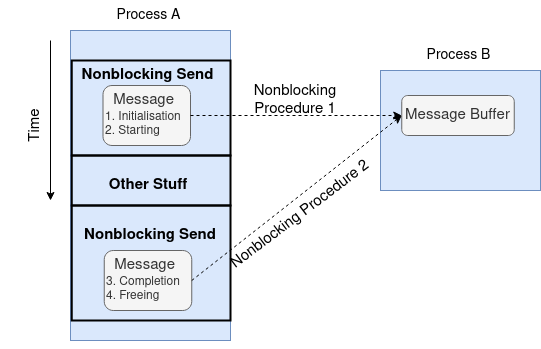
\includegraphics[width=0.6\textwidth]{NonBlocking_Send.png}
    \caption{The nonblocking send is split into two MPI procedures.}
\end{figure}
Notic\end{frame}

\begin{frame}[fragile]{Nonblocking Send Procedure 1}
\begin{block}{MPI$\_$ISEND}
MPI$\_$ISEND(\textbf{buf, count, datatype, dest, tag, comm})
\\
\begin{itemize}
\item[] IN \textbf{buf} \: \textit{starting address of buffer (choice)}\\
\item[] IN \textbf{count} \: \textit{number of entries in buffer (non-negative integer)}\\
\item[] IN \textbf{datatype} \: \textit{datatype of elements in send buffer (handle)}\\
\item[] IN \textbf{dest} \: \textit{rank of destination(integer)}\\
\item[] IN \textbf{tag} \: \textit{message tag (integer)}\\
\item[] IN \textbf{comm} \: \textit{communicator (handle)}\\
\item[] OUT \textbf{request} \: \textit{communication request(handle)}
\end{itemize}
\end{block}

C Binding
\rule{\textwidth}{1pt}
\scriptsize
\begin{minted}{C}
/* A buf message is sent from the calling rank to destination rank */
int MPI_Isend(const void *buf, int count, MPI_Datatype datatype, int dest,
int tag, MPI_Comm comm, MPI_Request *request)
\end{minted}
\rule{\textwidth}{1pt}
\end{frame}


\begin{frame}{MPI$\_$ISEND}
\begin{outline}
\1 The nonblocking send operation has the same communication modes as the blocking verson.

\1 The arguments
are the same as for MPI$\_$Send with the addition of a handle \textit{request}.
\2 The \textit{request} is an opaque objects to identify communication oper-
ations and match the operation that initiates the communication with the operation that
terminates it.
\2 That is, the \textit{request} handle is used in the nonblocking procedure 2.
\end{outline}
\end{frame}

\begin{frame}[fragile]{Nonblocking Procedure 2}
\begin{block}{MPI$\_$WAIT}
MPI$\_$WAIT(\textbf{request, status})
\\
\begin{itemize}
\item[] INOUT \textbf{request} \: \textit{communication request (handle)}
\item[] OUT   \textbf{status} \: \textit{status object (status)}
\end{itemize}
\end{block}

\rule{\textwidth}{1pt}
\scriptsize
\begin{minted}{C}
/* wait for nonblockcing procedure 1 to complete*/
int MPI_Wait(MPI_Request *request, MPI_Status *status)
\end{minted}
\rule{\textwidth}{1pt}

\begin{block}{MPI$\_$WAITALL}
MPI$\_$WAITALL(\textbf{count, array$\_$of$\_$requests, array$\_$of$\_$statuses})
\\
\begin{itemize}
\item[] IN \textbf{count} \: \textit{list length (non-negative integer)}
\item[] INOUT \textbf{request} \: \textit{communication request (handle)}
\item[] OUT   \textbf{status} \: \textit{status object (status)}
\end{itemize}
\end{block}
\rule{\textwidth}{1pt}
\scriptsize
\begin{minted}{C}
/* wait for a list of nonblockcing procedure 1 to complete*/
int MPI_Waitall(int count, MPI_Request array_of_requests[],
MPI_Status array_of_statuses[])
\end{minted}
\rule{\textwidth}{1pt}
\end{frame}


\begin{frame}{MPI$\_$WAIT}
\begin{outline}
\1 MPI$\_$WAIT returns when the operation identified by \textit{request} is complete.
\1 MPI$\_$WAITALL returns when all communication operations in the list are complete.
\1 What if we just want to check if a communication operation is complete rather than waiting for its completion?
\end{outline}    
\end{frame}


\begin{frame}[fragile]{}
\begin{block}{MPI$\_$TEST }
int MPI$\_$TEST(\textbf{request, flag, status})
\\
\begin{itemize}
\item[] INOUT \textbf{request} \: \textit{communication request (handle)}
\item[] OUT \textbf{flag} \: \textit{true if operation completed (logical)}
\item[] OUT   \textbf{status} \: \textit{status object (status)}
\end{itemize}
\end{block}

\rule{\textwidth}{1pt}
\scriptsize
\begin{minted}{C}
int MPI_Test(MPI_Request *request, MPI_Status *status)
\end{minted}
\rule{\textwidth}{1pt}

\begin{block}{MPI$\_$TESTALL}
MPI$\_$TESTALL(\textbf{count, array$\_$of$\_$requests, flag, array$\_$of$\_$statuses})
\\
\begin{itemize}
\item[] IN \textbf{count} \: \textit{list length (non-negative integer)}
\item[] INOUT \textbf{request} \: \textit{communication request (handle)}
\item[] OUT falg \: \textit{true if all of the operations are complete (logical)}
\item[] OUT   \textbf{status} \: \textit{status object (status)}
\end{itemize}
\end{block}
\rule{\textwidth}{1pt}
\scriptsize
\begin{minted}{C}
int MPI_Testall(int count, MPI_Request array_of_requests[], int *flag,
MPI_Status array_of_statuses[])
\end{minted}
\rule{\textwidth}{1pt}
\end{frame}


\begin{frame}{MPI$\_$IRECV}
\begin{figure}
    \centering
    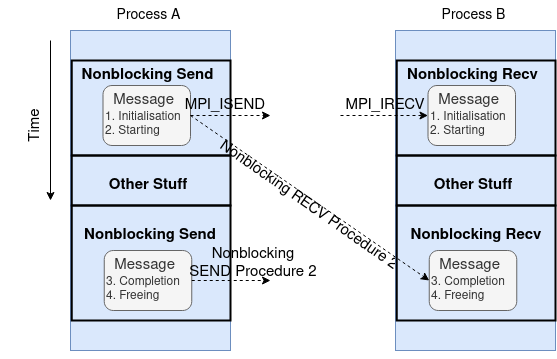
\includegraphics[width=0.6\textwidth]{NonBlocking_Recv.png}
    \caption{Nonblocking RECV may be posted before the matching send is initiated. Its completion does not indicate that the matching send operation has completed.}
\end{figure}
\end{frame}

\begin{frame}[fragile]{}
\begin{block}{MPI$\_$IRECV \cite{mpi40}}
MPI$\_$IRECV(\textbf{bug, count, datatype, source, tag, comm, request})
\\
\begin{itemize}
\item[] OUT \textbf{buf} \: \textit{starting address of buffer (choice)}\\
\item[] IN \textbf{count} \: \textit{number of entries in buffer (non-negative integer)}\\
\item[] IN \textbf{datatype} \: \textit{datatype of elements in send buffer (handle)}\\
\item[] IN \textbf{source} \: \textit{rank of destination(integer)}\\
\item[] IN \textbf{tag} \: \textit{message tag (integer)}\\
\item[] IN \textbf{comm} \: \textit{communicator (handle)}\\
\item[] OUT \textbf{request} \: \textit{communication request(handle)}
\end{itemize}
\end{block}
\rule{\textwidth}{1pt}
\scriptsize
\begin{minted}{C}
int MPI_Irecv(void *buf, int count, MPI_Datatype datatype, int source,
int tag, MPI_Comm comm, MPI_Request *request)
\end{minted}
\rule{\textwidth}{1pt}
\end{frame}

\begin{frame}{Overlapping Communication and Computation}
\begin{figure}
    \centering
    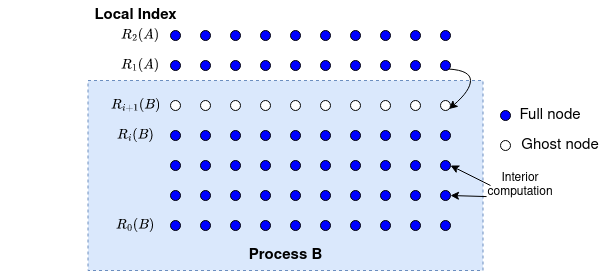
\includegraphics[width=0.9\textwidth]{Submesh_int.png}
    \caption{Jacobi method can perform on interior nodes independently without relying on communications. }
\end{figure}
\end{frame}

\begin{frame}[fragile]{Overlapping Communication and Computation}
\rule{\textwidth}{1pt}
\scriptsize
\begin{minted}{C}
/* Initiate sending the top and bottom row of full nodes*/
MPI_Isend(submesh[1], mesh_size, MPI_DOUBLE, lower, lowertag,\
MPI_COMM_WORLD, &bottom_bnd_requests[1]);

MPI_Isend(submesh[*ptr_rows-2], mesh_size, MPI_DOUBLE, upper, uppertag, \ 
MPI_COMM_WORLD, &top_bnd_requests[1]);

/* Jacobi method iterates on the interior full nodes */
Jacobi_int(ptr_rows, mesh_size, &submesh[0][0], &submesh_new[0][0], \ 
&subrhs[0][0], space);

/* Test the top and bottom row of ghost nodes */
MPI_Testall(2, top_bnd_requests, &top_flag, top_bnd_status);
MPI_Testall(2, bottom_bnd_requests, &bottom_flag, bottom_bnd_status;

/* Jacobi method iterates on top or bottom row of full nodes based \ 
on the testing results */
\end{minted}
\rule{\textwidth}{1pt}
See the complementary code for details.
\end{frame}

\begin{frame}{Exercise}
Rewrite the nonblocking send and receive such that it waits until the completion of both top and bottom rows of ghost nodes.
\end{frame}


\begin{frame}{Topic 1C: Persistent Communication}
\begin{figure}
    \centering
    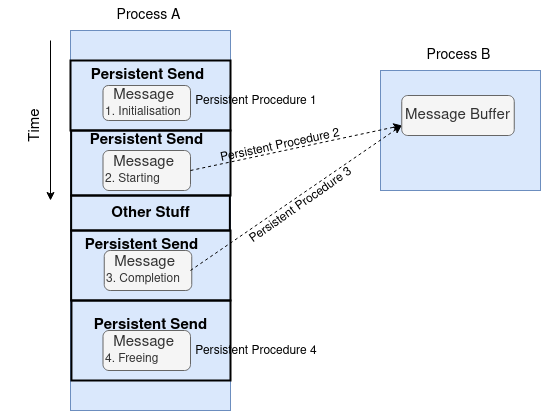
\includegraphics[width=0.8\textwidth]{Persistent_Send.png}
    \label{standard_send}
\end{figure}
\end{frame}



\begin{frame}{Topic 1C: Persistent Communication}
\begin{outline}
\1 A separate procedure for each of four stages.
\1 The same argument list is used in every single iteration and cumulatively creates overhead when get passed to communication controller repeatedly.
\1 Persistent communication allows the argument list to bind with the request once.
\end{outline}
\end{frame}

\begin{frame}[fragile]{Persistent Send Procedure 1}
\begin{block}{MPI$\_$SEND$\_$INIT}
MPI$\_$SEND$\_$INIT(\textbf{buf, count, datatype, dest, tag, comm, request})
\\
\begin{itemize}
\item[] IN \textbf{buf} \: \textit{starting address of buffer (choice)}\\
\item[] IN \textbf{count} \: \textit{number of entries in buffer (non-negative integer)}\\
\item[] IN \textbf{datatype} \: \textit{datatype of elements in send buffer (handle)}\\
\item[] IN \textbf{dest} \: \textit{rank of destination(integer)}\\
\item[] IN \textbf{tag} \: \textit{message tag (integer)}\\
\item[] IN \textbf{comm} \: \textit{communicator (handle)}\\
\item[] OUT \textbf{request} \: \textit{communication request(handle)}
\end{itemize}
\end{block}

C Binding
\rule{\textwidth}{1pt}
\scriptsize
\begin{minted}{C}
/* Create a persistent communication request */
int MPI_Send_init(const void *buf, int count, MPI_Datatype datatype, int dest,
int tag, MPI_Comm comm, MPI_Request *request)
\end{minted}
\rule{\textwidth}{1pt}
\end{frame}

\begin{frame}[fragile]{Persistent Send Procedure 2}
\begin{block}{MPI$\_$START}
MPI$\_$START(\textbf{ request})
\\
\begin{itemize}
\item[] OUT \textbf{request} \: \textit{communication request(handle)}
\end{itemize}
\end{block}

C Binding
\rule{\textwidth}{1pt}
\scriptsize
\begin{minted}{C}
/* Start a persistent communication request */
int MPI_Start(MPI_Request *request)
\end{minted}
\rule{\textwidth}{1pt}

\begin{block}{MPI$\_$STARTALL}
MPI$\_$STARTALL(\textbf{ count, array$\_$of$\_$request})
\\
\begin{itemize}
\item[] IN \textbf{count} \: \textit{list length (non-negative integer)}\\
\item[] OUT \textbf{request} \: \textit{communication request(handle)}
\end{itemize}
\end{block}

C Binding
\rule{\textwidth}{1pt}
\scriptsize
\begin{minted}{C}
/* Start a list of persistent communication requests */
int MPI_Startall(int count, MPI_Request array_of_requests[])
\end{minted}
\rule{\textwidth}{1pt}
\end{frame}

\begin{frame}{}
\begin{outline}
\1 MPI$\_$Send$\_$INIT creates a persistent communication request, which involves no communication.
\2 Communication that uses the persistent communication request is started by the procedure MPI$\_$Start. 
\end{outline}
\end{frame}

\begin{frame}{Persistent Send Procedure 3}
\begin{outline}
\1 This is a completion procedure, so we will use MPI$\_$WAIT, MPI$\_$TEST or their variations.
\end{outline}
\end{frame}


\begin{frame}[fragile]{Persistent Send Procedure 4}
\begin{block}{MPI$\_$REQUEST$\_$FREE }
MPI$\_$REQUEST$\_$FREE(\textbf{request})
\\
\begin{itemize}
\item[] OUT \textbf{request} \: \textit{communication request(handle)}
\end{itemize}
\end{block}

C Binding
\rule{\textwidth}{1pt}
\scriptsize
\begin{minted}{C}
/* Deallocate the persistent communication request */
int MPI_Request_free(MPI_Request *request)
\end{minted}
\rule{\textwidth}{1pt}
\end{frame}

\begin{frame}[fragile]{Overlapping Communication and Computation}
\rule{\textwidth}{1pt}
\scriptsize
\begin{minted}{C}
/* Initialise sending the  bottom row of full nodes */
MPI_Send_init(submesh[1], mesh_size, MPI_DOUBLE, lower, lowertag,\ 
MPI_COMM_WORLD, &bottom_bnd_requests[1]);

for (int iter = 0; iter < 100; iter++){
/* Activate the communication request */
MPI_Startall(2, bottom_bnd_requests);
/* Jacobi method iterates on the interior full nodes */
Jacobi_int(ptr_rows, mesh_size, &submesh[0][0], &submesh_new[0][0], \ 
&subrhs[0][0], space);

/* Test the top and bottom row of ghost nodes */
MPI_Testall(2, bottom_bnd_requests, &top_flag, bottom_bnd_status);
Jacobi_bottom(ptr_rows, mesh_size, &submesh[0][0], &submesh_new[0][0], &subrhs[0][0], space);

/* Jacobi method iterates on bottom row of full nodes based \ 
on the testing results */
MPI_Waitall(2, bottom_bnd_requests, bottom_bnd_status);

}
/* Free the request handle */
MPI_Request_free(bottom_bnd_request);
\end{minted}
\rule{\textwidth}{1pt}
\end{frame}

\begin{frame}{Exercise}
Refactor the nonblocking communication code to use persistence communication.
\end{frame}

\begin{frame}{Showcase: 2D unstructured grid}
\begin{figure}
    \centering
    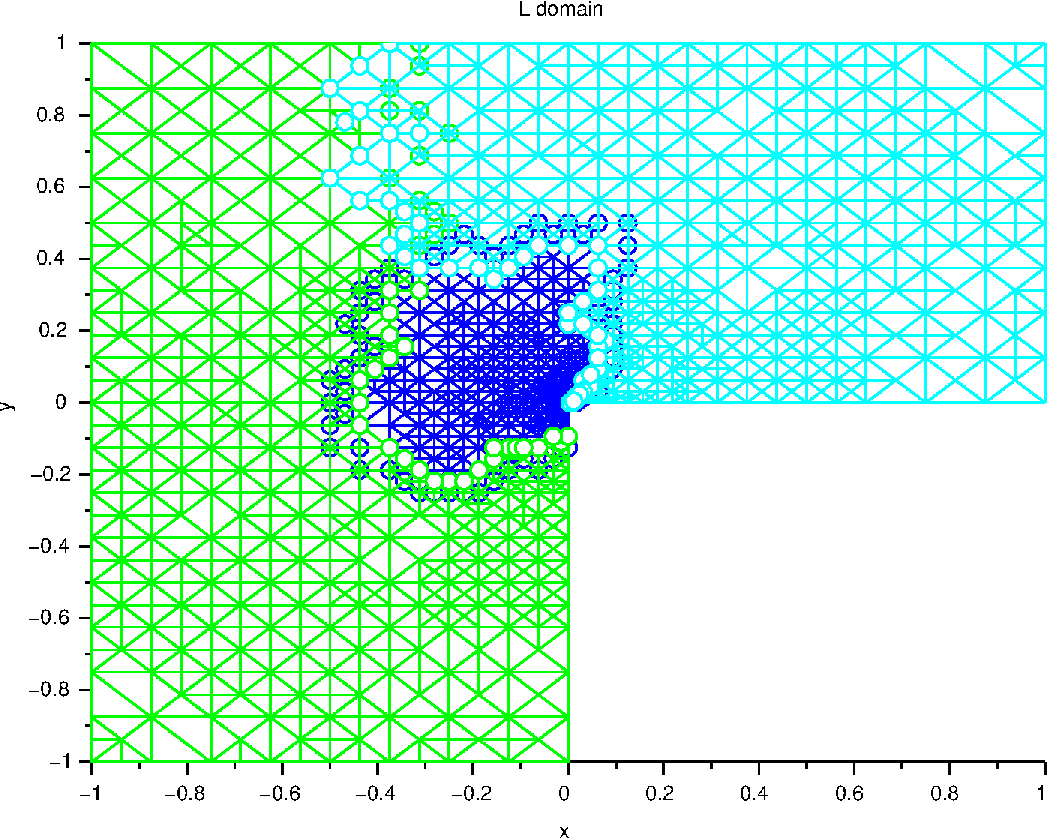
\includegraphics[width=0.8\textwidth]{L_par_whole_2D.pdf}
    \caption{2D adaptively refine grid distributed over three processors  \cite{stals2019algorithm}. }
\end{figure}
\end{frame}


\section{Collective communication}
\begin{frame}{}
$$\textbf{Topic 2: Collective Communication}$$
\end{frame}

\begin{frame}{Topic 2: Collective Communication}
\begin{figure}
    \centering
    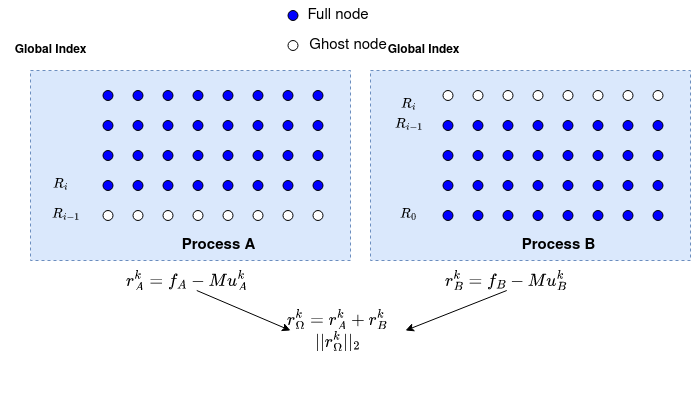
\includegraphics[width=0.8\textwidth]{Submesh_Res.png}
    \caption{Collecting local residuals from each individual process to calculate the global residual.}
    \label{standard_send}
\end{figure}
\end{frame}





\begin{frame}{Topic 2: Collective Communication}
\begin{block}{Definition}
Collective communication is defined as communication that involves a group or groups of processes.
\end{block}
\begin{outline}
    \1 \textbf{All to All}: MPI$\_$ALLREDUCE, MPI$\_$BARRIER, MPI$\_$ALLREDUCE$\_$INIT,etc.
    \1 \textbf{All to One}: MPI$\_$GATHER, MPI$\_$REDUCE, etc.
    \1 \textbf{One to All}: MPI$\_$SCATTER, MPI$\_$BCAST, etc.
    \1 \textbf{Other}: MPI$\_$SCAN
\end{outline}
\end{frame}


\begin{frame}{MPI$\_$BCAST}
\begin{figure}
    \centering
    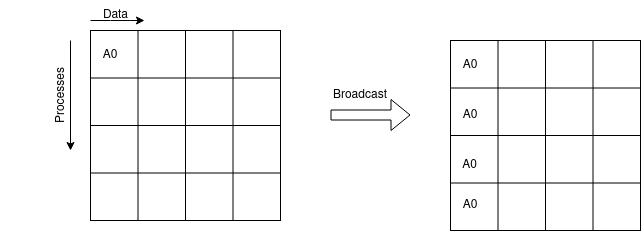
\includegraphics[width=0.8\textwidth]{broadcast.png}
    \caption{Each row of boxes represents data locations in one process. Initially
just the first process contains the data $A_0$ , but after the broadcast all processes contain it \cite{mpi40}.}
    \label{fork}
\end{figure}
\end{frame}

\begin{frame}[fragile]{MPI$\_$BCAST}
\begin{block}{MPI$\_$BCAST}
MPI$\_$BCAST(\textbf{buffer, count, datatype, root, comm})
\\
\begin{itemize}
\item[] INOUT \textbf{buffer} \: \textit{starting address of buffer (choice)}\\
\item[] IN \textbf{count} \: \textit{number of entries in buffer (non-negative integer)}\\
\item[] IN \textbf{datatype} \: \textit{datatype of buffer (handle)}\\
\item[] IN \textbf{root} \: \textit{rank of broadcast root (integer)}\\
\item[] IN \textbf{comm} \: \textit{communicator (handle)}
\end{itemize}
\end{block}

C Binding
\rule{\textwidth}{1pt}
\scriptsize
\begin{minted}{C}
/* Copy root's buffer into all other processes that are member of
the comm group */
int MPI_Bcast(void *buffer, int count, MPI_Datatype datatype, int root,
MPI_Comm comm)
\end{minted}
\rule{\textwidth}{1pt}
\end{frame}
    
\begin{frame}{MPI$\_$BCAST}
\begin{itemize}
    \item All processes in the communicator must be involved,
    \item Count must be equal between the root and all other processes,\\
    \item Comm can be an inter-communicator,
    \item The order of execution of the collective operation should prevent deadlocking
\end{itemize}
\end{frame}

\begin{frame}{MPI$\_$REDUCE}
\begin{figure}
    \centering
    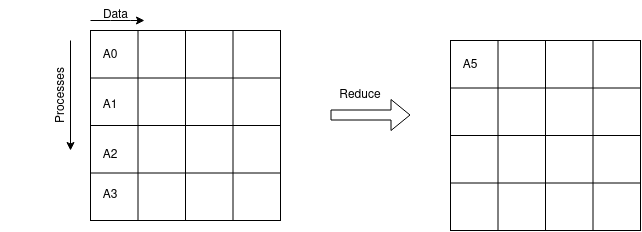
\includegraphics[width=0.8\textwidth]{Reduce.png}
    \caption{A global reduce operation performs across all members of the group and returns the result of the reduction to one member of the group \cite{mpi40}.}
    \label{fork}
\end{figure}
\end{frame}

\begin{frame}[fragile]{}
\begin{block}{MPI$\_$REDUCE}
MPI$\_$REDUCE(\textbf{sendbuf, recvbuf, count, datatype, op,  root, comm})
\\
\begin{itemize}
\item[] IN \textbf{sendbuf} \: \textit{address of send buffer (choice)}\\
\item[] OUT \textbf{recvbuf} \: \textit{address of receive buffer (choice, significant only at
root)}\\
\item[] IN \textbf{count} \: \textit{number of elements in send buffer (non-negative
integer)}\\
\item[] IN \textbf{datatype} \: \textit{datatype of elements of send buffer (handle)}\\
\item[] IN \textbf{op} \: \textit{reduce operation (handle)}\\
\item[] IN \textbf{root} \: \textit{rank of root process (integer)}\\
\item[] IN \textbf{comm} \: \textit{communicator (handle)}
\end{itemize}
\end{block}
\rule{\textwidth}{1pt}
\end{frame}



\begin{frame}[fragile]{Reduce the residuals to one process}
\rule{\textwidth}{1pt}
\scriptsize
\begin{minted}{C}
/* get local residual from each process */
double residual, tot_res;
residual  = local_l2_residual(ptr_rows, mesh_size, space, &submesh[0][0], \
subrhs[0][0]);
    
/* sum res from all processes and calculate l2 norm */
MPI_Reduce(&residual, &tot_res, 1, MPI_DOUBLE, MPI_SUM, 0, MPI_COMM_WORLD);
if (rank == 0){
    tot_res = sqrt(tot_res);
    printf("Residual1  %f\n",  tot_res); 
    }
\end{minted}
\rule{\textwidth}{1pt}
\end{frame}

\begin{frame}{Predefined Reduction Operations}
\begin{outline}
\1 MPI$\_$MAX: maximum
\1 MPI$\_$MIN: minimum
\1 MPI$\_$SUM: sum
\1 MPI$\_$PROD: product
\1 MPI$\_$MAXLOC: max value and location
\1 MPI$\_$MINLOC: min value and location
\1 and a few more bit-wise operators.
\end{outline}

User-defined reduction operation is also possible.
\end{frame}


\begin{frame}{MPI$\_$ALLREDUCE}
\begin{figure}
    \centering
    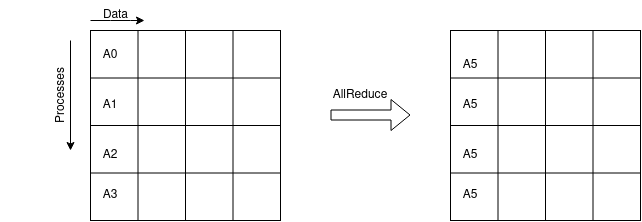
\includegraphics[width=0.8\textwidth]{Allreduce.png}
    \caption{MPI$\_$ALLREDUCE = MPI$\_$REDUCE + MPI$\_$BCAST. }
\end{figure}
\end{frame}


\begin{frame}{MPI$\_$GATHER and  MPI$\_$SCATTER}
\begin{figure}
    \centering
    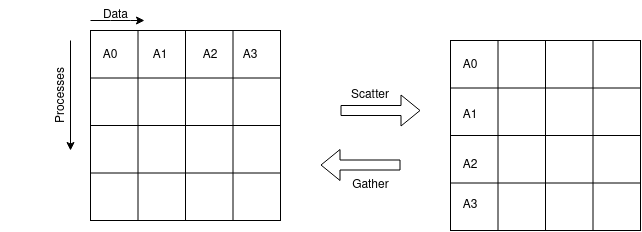
\includegraphics[width=0.8\textwidth]{gather-scatter.png}
    \caption{Gather: Each process contains the data $A_i$ and sends to the root process. The root process receive the messages and store them in the rank order\cite{mpi40}.}
    \label{fork}
\end{figure}
\end{frame}

\begin{frame}[fragile]{}
\begin{block}{MPI$\_$Gather}
MPI$\_$Gather(\textbf{sendbuf, sendcount, sendtype, recvbug, recvcount,  recvcount, recvtype, root, comm})
\\
\begin{itemize}
\item[] IN \textbf{sendbuf} \: \textit{address of send buffer (choice)}\\
\item[] IN \textbf{sendcount} \: \textit{number of elements in send buffer (non-negative integer)}\\
\item[] IN \textbf{sendtype} \: \textit{datatype of send buffer elements (handle)}\\
\item[] OUT \textbf{recvbuf} \: \textit{address of receive buffer (choice, significant only at root)}\\
\item[] IN \textbf{recvcount} \: \textit{number of elements for any single receive}\\
\item[] IN \textbf{recvtype} \: \textit{datatype of recv buffer elements (handle, significant only at root)}\\
\item[] IN \textbf{root} \: \textit{rank of root process (integer)}\\
\item[] IN \textbf{comm} \: \textit{communicator (handle)}
\end{itemize}
\end{block}
\rule{\textwidth}{1pt}
\end{frame}




\begin{frame}[fragile]{MPI$\_$Gather}
\rule{\textwidth}{1pt}
\scriptsize
\begin{minted}{C}
/* All processes send the message to the root process and the root 
process stores them in rank order*/
int MPI_Gather(const void *sendbuf, int sendcount, MPI_Datatype sendtype,
void *recvbuf, int recvcount, MPI_Datatype recvtype, int root,
MPI_Comm comm)
\end{minted}
\rule{\textwidth}{1pt}
\end{frame}

\begin{frame}{Non-associative operations}
In a floating-point system $\mathcal{F}$, the multiplication and addition operations are not associative. That is
\begin{align*}
    (a+b)+c \ne a+(b+c)\quad \text{for } a,b, c\in \mathcal{F}.
\end{align*}

Implying that the order of the operands may be important for reproducibility.
\end{frame}

\begin{frame}{Exercise}
Replace the $MPI\_REDUCE$ call with $MPI\_GATHER$ to collect residuals to a root process in rank order. Then calculate the total residual from the root process.
\end{frame}

\begin{frame}{Collective communication}
\begin{outline}
\1 MPI$\_$REDUCE, MPI$\_$ALLREDUCE, MPI$\_$GATHER, MPI$\_$SCATTER, MPI$\_$BCAST are also blocking procedures.
\1 There are non-blocking versions of those procedures following the same definition of the nonblocking operation that we discussed before.

\1 There also are persistent versions of those procedures following the same definition of the persistent operation that we discussed before.
\end{outline}
\end{frame}



\section{One-sided Communication}
\begin{frame}{}
$$\textbf{Topic 3: One-sided Communication}$$
\end{frame}


\begin{frame}{One-sided communication}
\begin{block}{Definition}
One-sided communication aka. Remote Memory Access (RMA) reads, writes, updates and swaps data at a remote process without a matching receive or send. 
\end{block}
\end{frame}

\begin{frame}{}
\begin{figure}
    \centering
    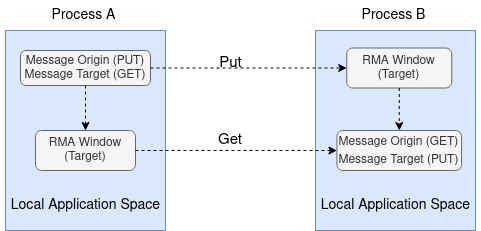
\includegraphics[width=0.6\textwidth]{MPI_WIN.png}
    \caption{Transfer data from Origin to Target by One-sided Put and Get respectively.}
    \label{fork}
\end{figure}
\end{frame}


\begin{frame}{Why one-sided communication?}
\begin{outline}
    \1 Asymmetricity between regular SEND and RECV.
    \2 Message parameters are all available on one side.
    \1 Avoids distributing transfer parameters.
    \2 By creating a window object that is accessible to processes at remote.
\end{outline}
\end{frame}

\begin{frame}[fragile]{}
\begin{block}{MPI$\_$WIN$\_$CREATE}
MPI$\_$WIN$\_$CREATE(\textbf{base, size, disp$\_$unit, info,comm,  win})
\\
\begin{itemize}
\item[] IN \textbf{base} \: \textit{initial address of window (choice)}\\
\item[] IN \textbf{size} \: \textit{size of window in bytes (non-negative integer)}\\
\item[] IN \textbf{disp$\_$unit} \: \textit{local unit size for displacements, in bytes (positive integer)}
\item[] IN \textbf{info} \: \textit{info argument (handle)}\\
\item[] IN  \textbf{comm} \: \textit{intra-communicator (handle)} \\
\item[] OUT \textbf{window} \: \textit{window object (handle)}
\end{itemize}
\end{block}

C Binding
\rule{\textwidth}{1pt}
\scriptsize
\begin{minted}{C}
/* create a local window object */
int MPI_Win_create(void *base, MPI_Aint size, int disp_unit, MPI_Info info,
MPI_Comm comm, MPI_Win *win)
\end{minted}
\rule{\textwidth}{1pt}
\end{frame}


\begin{frame}{MPI$\_$WIN$\_$CREATE}
\begin{outline}
    \1 Creating local RMA window is a collective call - it must be called on every process in the group.
    \1 This call does not allocate memory. The local memory needs to be allocated separately to be used in RMA operation.
\end{outline}
\end{frame}



\begin{frame}{Communicate ghost row through MPI$\_$PUT}
\begin{figure}
    \centering
    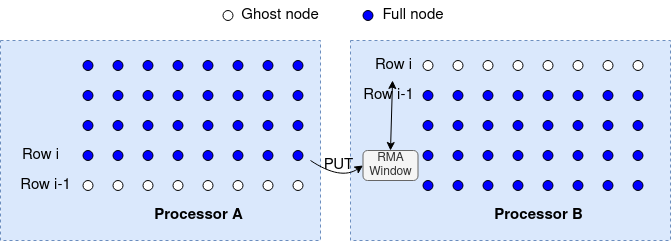
\includegraphics[width=\textwidth]{Submesh_Win.png}
    \caption{The $i$th row of full nodes in $A$ is put into the local RMA window in $B$.}
    \label{fork}
\end{figure}
\end{frame}

\begin{frame}[fragile]{}
\begin{block}{MPI$\_$PUT}
MPI$\_$PUT (\textbf{origin$\_$addr, origin$\_$count, orgin$\_$datatype, target$\_$rank, target$\_$disp, target$\_$count, target$\_$datatype,win})
\\
\begin{itemize}
\item[] IN \textbf{origin$\_$addr} \: \textit{initial address of origin buffer (choice)}\\
\item[] IN \textbf{origin$\_$count} \: \textit{number of entries in origin buffer (non-negative integer)}\\
\item[] IN \textbf{origin$\_$datatype} \: \textit{datatype of each entry in origin buffer (handle)}
\item[] IN \textbf{target$\_$rank} \: \textit{rank of target (non-negative integer)}\\
\item[] IN  \textbf{target$\_$disp} \: \textit{displacement from start of window to target buffer (non-negative integer)} \\
\item[] IN \textbf{target$\_$count} \: \textit{number of entries in target buffer (non-negative integer)}\\
\item[] IN \textbf{target$\_$datatype} \: \textit{datatype of each entry in target buffer (handle)} \\
\item[] OUT \textbf{window} \: \textit{window object (handle)}
\end{itemize}
\end{block}
\end{frame}

\begin{frame}[fragile]{MPI$\_$PUT}
C Binding
\rule{\textwidth}{1pt}
\scriptsize
\begin{minted}{C}
/* create a local window object */
int MPI_Put(const void *origin_addr, int origin_count,
MPI_Datatype origin_datatype, int target_rank, MPI_Aint target_disp, 
int target_count, MPI_Datatype target_datatype, MPI_Win win)
\end{minted}
\rule{\textwidth}{1pt}
\end{frame}

\begin{frame}{MPI$\_$PUT: argument list explained}
\begin{figure}
    \centering
    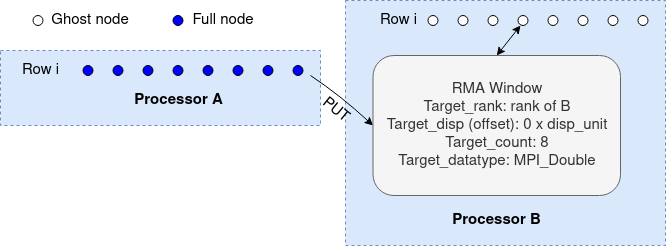
\includegraphics[width=\textwidth]{RMA_window.png}
    \caption{The $i$th row of full nodes in $A$ is put directly into the local RMA window in $B$.}
    \label{fork}
\end{figure}
\end{frame}


\begin{frame}{RMA Window}
\begin{outline}
\1 target$\_$disp is determined by the disp$\_$unit specified in MPI$\_$WIN$\_$CREATE. 
\1 Multiple MPI$\_$PUT operations can be performed on a RMA window.
\1 MPI$\_$PUT's behaviour is nonblocking alike a combination of MPI$\_$ISEND and MPI$\_$IRECV.
\2 It needs another MPI call to complete.
\end{outline}
\end{frame}



\begin{frame}[fragile]{}
\begin{block}{MPI$\_$WIN$\_$FENCE}
MPI$\_$WIN$\_$FENCE (\textbf{assert, win})
\\
\begin{itemize}
\item[] IN \textbf{assert} \: \textit{program assertion (integer)}\\
\item[] IN \textbf{win} \: \textit{window object (handle)}
\end{itemize}
\end{block}
C Binding
\rule{\textwidth}{1pt}
\scriptsize
\begin{minted}{C}
/* create a local window object */
int MPI_Win_fence(int assert, MPI_Win win)
\end{minted}
\rule{\textwidth}{1pt}

\begin{block}{Assertions}
The \textit{assert} flag is used to provide assertions on the context of the call that may be used to optimise performance.
\end{block}
\end{frame}

\begin{frame}{MPI$\_$WIN$\_$FENCE}
\begin{outline}
\1 MPI$\_$WIN$\_$FENCE not only completes but also starts an \textit{access epoch} at an origin process and an \textit{exposure epoch} at an target process.
\2 Access/Exposure epochs is the time when the local window is available for access.
\2 "Switch" between origin and target.
\end{outline}
\end{frame}
\begin{frame}{MPI$\_$WIN$\_$FENCE}
\begin{figure}
    \centering
    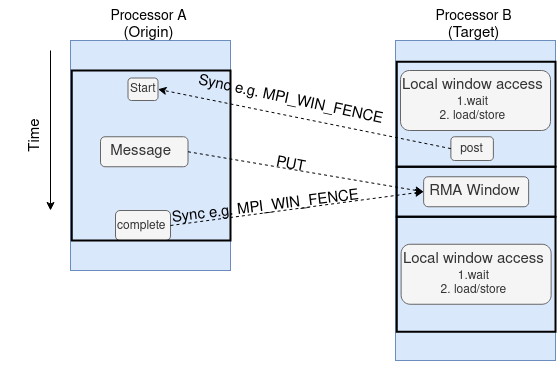
\includegraphics[width=0.8\textwidth]{RMA_Fence.png}
    \caption{Active target communication where MPI$\_$WIN$\_$FENCE is used for synchronisation \cite{mpi40}.}
    \label{fork}
\end{figure}
\end{frame}

\begin{frame}[fragile]{One-sided communication}
\rule{\textwidth}{1pt}
\scriptsize
\begin{minted}{C}
/* create a local window object */
MPI_Win upper_win;
double *upper_bnd;
MPI_Alloc_mem(sizeof(double )*mesh_size, MPI_INFO_NULL, &upper_bnd);
MPI_Win_create(upper_bnd, mesh_size *sizeof(double), sizeof(double),\
               MPI_INFO_NULL, MPI_COMM_WORLD, &upper_win);
               
/* start access/exposure epoch */
MPI_Win_fence(0, upper_win);

/* RMA operation */
MPI_Put(submesh[1], mesh_size, MPI_DOUBLE, \ 
lower, 0, mesh_size, MPI_DOUBLE, upper_win);

/* complete access/exposure epoch */
MPI_Win_fence(0, upper_win);
\end{minted}
\rule{\textwidth}{1pt}
\end{frame}

\begin{frame}{Exercise}
Transfer both top and bottom row of ghost nodes in one RMA window by carefully specifying the target$\_$disp argument in MPI$\_$PUT.
\end{frame}

\section{MPI Profiler}
\begin{frame}{}
$$ \textbf{Topic 5: MPI Profiling}$$
\end{frame}
   
\begin{frame}{Foundation: MPI Profiling Interface}
\begin{block}{PMPI$\_$ Prefix \cite{mpi40}}
PMPI$\_$ prefix defines an alternate entry point name for each MPI function.
\end{block}
Example: MPI$\_$SEND, PMPI$\_$SEND.
\end{frame}

\begin{frame}{Foundation: MPI Profiling Interface}
\begin{outline}
\1 The functions with PMPI$\_$ prefix have the same functionality as the MPI version.
\2 This allows profiling tools to intercept applications' MPI function calls and do surrounding profiling work.
\end{outline}
\begin{block}{}
User's MPI call$\xRightarrow[]{intercepted}$Profiler Library$\xRightarrow[]{internal\; call}$PMPI call
\end{block}
\end{frame}

\begin{frame}[fragile]{A simple profiler implementation \cite{mpi40}}
\rule{\textwidth}{1pt}
\scriptsize
\begin{minted}{C}
static int totalBytes = 0;
static double totalTime = 0.0;

int MPI_Send(const void* buffer, int count, MPI_Datatype datatype,
int dest, int tag, MPI_Comm comm){
double tstart = MPI_Wtime();
int size;
/* call PMPI internally */
int result = PMPI_Send(buffer,count,datatype,dest,tag,comm);
/* surrounding profiling work */
totalTime += MPI_Wtime() - tstart;
MPI_Type_size(datatype, &size);
totalBytes += count*size;
return result;}
\end{minted}
\rule{\textwidth}{1pt}
When this profiler library  is linked it will intercept MPI$\_$SEND call from users' application to count elapsed time and the amount of data.  
\end{frame}

\begin{frame}{mpiP}
\begin{outline}
\1 mpiP is a light-weight profiling library for MPI applications.
\2 Build on top of PMPI.
\2 Measures the entire MPI application from MPI$\_$INIT to MPI$\_$FINALIZE
\1 mpiP 3.4 is available on Gadi by module load.
\end{outline}
\end{frame}




\begin{frame}{Exercise}

Using mpiP to measure the speedup for blocking, nonblocking and one-sided communication codes.    
\end{frame}


\section{MPI-IO}
\begin{frame}{}
$$\textbf{Topic 6: Basic MPI-IO}$$
\end{frame}

\begin{frame}{General IO operations on Gadi}
\begin{outline}
\1 Reasonable number of files under per parent directory to avoid lock contention - 10k-ish.
\1 Use striping file for parallel access for very large files.
\1 Calculate input/output data size. Read/write large size of data (>0.5 MB) if possible.

\footnotesize\textit{Courtesy of Kim}
\end{outline}
\end{frame}

\begin{frame}{}
\begin{figure}
    \centering
    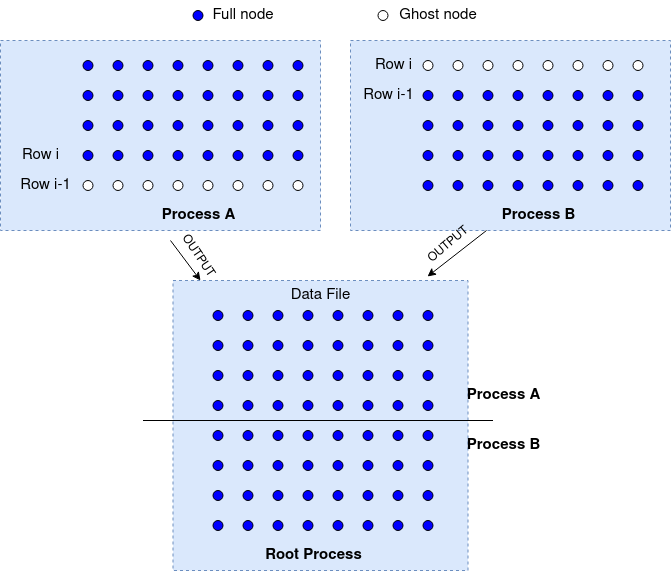
\includegraphics[width=0.65\textwidth]{Submesh_IO.png}
    \caption{Output submeshes from their local processes to a single file.}
    \label{fork}
\end{figure}
\end{frame}

\begin{frame}{Parallel IO}
\begin{outline}
\1 With Posix-IO,
\2 each process writes data to individual files or
\2 one process gathers all data and output a single file.
\1 With MPI-IO,
\2 multiple processes concurrently write to a single file.  
\end{outline}

\begin{block}{}
Of course, the parallel IO capability won't be possible without parallel file system support. On Gadi, it is our lustre file system.
\end{block}
\end{frame}

\begin{frame}{Basic MPI-IO}
\begin{outline}
\1 Open the file.
\1 Write to/read from the file.
\1 Close the file.
\end{outline}
\end{frame}

\begin{frame}[fragile]{Open the file}
\begin{block}{MPI$\_$FILE$\_$OPEN \cite{mpi40}}
MPI$\_$FILE$\_$OPEN(\textbf{comm, filename, amode, info, fh})
\\
\begin{itemize}
\item[] IN \textbf{comm} \: \textit{initial communicator (handle)}\\
\item[] IN \textbf{filename} \: \textit{name of file to open (string)}\\
\item[] IN \textbf{amode} \: \textit{file access mode (integer)}
\item[] IN \textbf{info} \: \textit{info object (handle)}\\
\item[] OUT  \textbf{fh} \: \textit{new file handle(handle)} \\
\end{itemize}
\end{block}

C Binding
\rule{\textwidth}{1pt}
\scriptsize
\begin{minted}{C}
/* open the file collectively */
int MPI_File_open(MPI_Comm comm, const char *filename, int amode,
MPI_Info info, MPI_File *fh)
\end{minted}
\rule{\textwidth}{1pt}
\end{frame}

\begin{frame}{MPI$\_$FILE$\_$OPEN}
\begin{outline}
\1 The call is a collective routine.
\2 All process in the comm group must provide the same amode
\3 MPI$\_$MODE$\_$CREATE: create the file if it does not exist;
\3 MPI$\_$MODE$\_$WRONLY: write only;
\3 MPI$\_$MODE$\_$RDONLY: read only;
\3 and many more.
\end{outline}
\end{frame}

\begin{frame}[fragile]{Close the file}
\begin{block}{MPI$\_$FILE$\_$CLOSE \cite{mpi40}}
MPI$\_$FILE$\_$CLOSE(\textbf{fh})
\\
\begin{itemize}
\item[] INOUT  \textbf{fh} \: \textit{file handle (handle)} \\
\end{itemize}
\end{block}

C Binding
\rule{\textwidth}{1pt}
\scriptsize
\begin{minted}{C}
/* close the file collectively */
int MPI_File_close(MPI_File *fh)
\end{minted}
\rule{\textwidth}{1pt}
\end{frame}

\begin{frame}[fragile]{Write to the file}
\begin{block}{MPI$\_$FILE$\_$WRITE$\_$AT \cite{mpi40}}
MPI$\_$FILE$\_$WRITE$\_$AT(\textbf{fh, offset, buf, count, datatype, status})
\\
\begin{itemize}
\item[] INOUT \textbf{fh} \: \textit{file handle (handle)}\\
\item[] IN \textbf{offset} \: \textit{file offset (integer)}\\
\item[] OUT \textbf{buf} \: \textit{initial address of buffer (choice)}
\item[] IN \textbf{count} \: \textit{number of elements in buffer (integer)}\\
\item[] IN \textbf{datatype} \: \textit{datatype of each buffer elemeent (handle)} \\
\item[] OUT  \textbf{status} \: \textit{status object (status)} \\
\end{itemize}
\end{block}

C Binding
\rule{\textwidth}{1pt}
\scriptsize
\begin{minted}{C}
/* writees a file beginning at the position specified by offset */
int MPI_File_read_at(MPI_File fh, MPI_Offset offset, void *buf, int count,
MPI_Datatype datatype, MPI_Status *status)
\end{minted}
\rule{\textwidth}{1pt}
\end{frame}

\begin{frame}{MPI$\_$FILE$\_$WRITE$\_$AT}
\begin{figure}
    \centering
    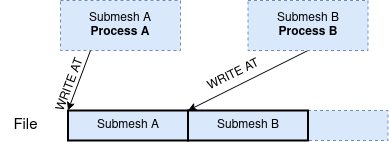
\includegraphics[width=0.65\textwidth]{File-IO.drawio.png}
    \caption{Each process writes at the offset position of the common file.}
    \label{fork}
\end{figure}
\end{frame}

\begin{frame}{MPI$\_$FILE$\_$WRITE$\_$AT}
\begin{outline}
\1 The call is noncollective. The collective version is defined with $\_ALL$ suffix.
\1 The call writes unformatted binary file.
\end{outline}
\end{frame}

\begin{frame}[fragile]{Basic MPI-IO}
\rule{\textwidth}{1pt}
\scriptsize
\begin{minted}{C}
/* create a local window object */
MPI_File fp;
MPI_Offset offset; 
MPI_File_open(MPI_COMM_WORLD, file_name, MPI_MODE_CREATE|MPI_MODE_WRONLY,\ 
MPI_INFO_NULL, &fp);
int count;
/* process contains the top mesh */
if (rank ==(cells -1)){
    count = mesh_size * (*ptr_rows -1);
    offset=  (mesh_size * (int_rows +1 )) * sizeof(double) + \
    (rank-1)*(mesh_size * int_rows) * sizeof(double);
    MPI_File_write_at(fp, offset, &submesh[1][0], count, MPI_DOUBLE, &IO_status );
}
/* process contains the bottom mesh */
else if (rank == 0 ) {
    count =  mesh_size * (*ptr_rows -1);
    offset = 0;
    MPI_File_write_at(fp, offset, &submesh[0][0], count, MPI_DOUBLE, &IO_status);
}
/* processes contain the rest of middle mesh */
else{
/* IO */
}
\end{minted}
\rule{\textwidth}{1pt}
\end{frame}





\begin{frame}[allowframebreaks]
        \frametitle{References}
        \bibliographystyle{amsalpha}
        \bibliography{mpi.bib}
\end{frame}





\begin{frame}{Thank you!}
$$\textbf{Please help us improve!}$$

\url{https://anu.au1.qualtrics.com/jfe/form/SV_0BRRQvSz5oiwOqO}
\end{frame}

\end{document}
